\documentclass[]{DissertateCUNY}
\usepackage{lmodern}
\usepackage{amssymb,amsmath}
\usepackage{ifxetex,ifluatex}
\usepackage{fixltx2e} % provides \textsubscript
\ifnum 0\ifxetex 1\fi\ifluatex 1\fi=0 % if pdftex
  \usepackage[T1]{fontenc}
  \usepackage[utf8]{inputenc}
\else % if luatex or xelatex
  \ifxetex
    \usepackage{mathspec}
  \else
    \usepackage{fontspec}
  \fi
  \defaultfontfeatures{Ligatures=TeX,Scale=MatchLowercase}
    \setmainfont[]{Times New Roman}
\fi
% use upquote if available, for straight quotes in verbatim environments
\IfFileExists{upquote.sty}{\usepackage{upquote}}{}
% use microtype if available
\IfFileExists{microtype.sty}{%
\usepackage{microtype}
\UseMicrotypeSet[protrusion]{basicmath} % disable protrusion for tt fonts
}{}
\usepackage[top=1in,bottom=1in,right=1in,left=1in]{geometry}
\usepackage{hyperref}
\hypersetup{unicode=true,
            pdftitle={Memory-guided selective attention},
            pdfauthor={Nicholaus P. Brosowsky},
            pdfborder={0 0 0},
            breaklinks=true}
\urlstyle{same}  % don't use monospace font for urls
\usepackage{color}
\usepackage{fancyvrb}
\newcommand{\VerbBar}{|}
\newcommand{\VERB}{\Verb[commandchars=\\\{\}]}
\DefineVerbatimEnvironment{Highlighting}{Verbatim}{commandchars=\\\{\}}
% Add ',fontsize=\small' for more characters per line
\usepackage{framed}
\definecolor{shadecolor}{RGB}{248,248,248}
\newenvironment{Shaded}{\begin{snugshade}}{\end{snugshade}}
\newcommand{\AlertTok}[1]{\textcolor[rgb]{0.94,0.16,0.16}{#1}}
\newcommand{\AnnotationTok}[1]{\textcolor[rgb]{0.56,0.35,0.01}{\textbf{\textit{#1}}}}
\newcommand{\AttributeTok}[1]{\textcolor[rgb]{0.77,0.63,0.00}{#1}}
\newcommand{\BaseNTok}[1]{\textcolor[rgb]{0.00,0.00,0.81}{#1}}
\newcommand{\BuiltInTok}[1]{#1}
\newcommand{\CharTok}[1]{\textcolor[rgb]{0.31,0.60,0.02}{#1}}
\newcommand{\CommentTok}[1]{\textcolor[rgb]{0.56,0.35,0.01}{\textit{#1}}}
\newcommand{\CommentVarTok}[1]{\textcolor[rgb]{0.56,0.35,0.01}{\textbf{\textit{#1}}}}
\newcommand{\ConstantTok}[1]{\textcolor[rgb]{0.00,0.00,0.00}{#1}}
\newcommand{\ControlFlowTok}[1]{\textcolor[rgb]{0.13,0.29,0.53}{\textbf{#1}}}
\newcommand{\DataTypeTok}[1]{\textcolor[rgb]{0.13,0.29,0.53}{#1}}
\newcommand{\DecValTok}[1]{\textcolor[rgb]{0.00,0.00,0.81}{#1}}
\newcommand{\DocumentationTok}[1]{\textcolor[rgb]{0.56,0.35,0.01}{\textbf{\textit{#1}}}}
\newcommand{\ErrorTok}[1]{\textcolor[rgb]{0.64,0.00,0.00}{\textbf{#1}}}
\newcommand{\ExtensionTok}[1]{#1}
\newcommand{\FloatTok}[1]{\textcolor[rgb]{0.00,0.00,0.81}{#1}}
\newcommand{\FunctionTok}[1]{\textcolor[rgb]{0.00,0.00,0.00}{#1}}
\newcommand{\ImportTok}[1]{#1}
\newcommand{\InformationTok}[1]{\textcolor[rgb]{0.56,0.35,0.01}{\textbf{\textit{#1}}}}
\newcommand{\KeywordTok}[1]{\textcolor[rgb]{0.13,0.29,0.53}{\textbf{#1}}}
\newcommand{\NormalTok}[1]{#1}
\newcommand{\OperatorTok}[1]{\textcolor[rgb]{0.81,0.36,0.00}{\textbf{#1}}}
\newcommand{\OtherTok}[1]{\textcolor[rgb]{0.56,0.35,0.01}{#1}}
\newcommand{\PreprocessorTok}[1]{\textcolor[rgb]{0.56,0.35,0.01}{\textit{#1}}}
\newcommand{\RegionMarkerTok}[1]{#1}
\newcommand{\SpecialCharTok}[1]{\textcolor[rgb]{0.00,0.00,0.00}{#1}}
\newcommand{\SpecialStringTok}[1]{\textcolor[rgb]{0.31,0.60,0.02}{#1}}
\newcommand{\StringTok}[1]{\textcolor[rgb]{0.31,0.60,0.02}{#1}}
\newcommand{\VariableTok}[1]{\textcolor[rgb]{0.00,0.00,0.00}{#1}}
\newcommand{\VerbatimStringTok}[1]{\textcolor[rgb]{0.31,0.60,0.02}{#1}}
\newcommand{\WarningTok}[1]{\textcolor[rgb]{0.56,0.35,0.01}{\textbf{\textit{#1}}}}
\usepackage{graphicx,grffile}
\makeatletter
\def\maxwidth{\ifdim\Gin@nat@width>\linewidth\linewidth\else\Gin@nat@width\fi}
\def\maxheight{\ifdim\Gin@nat@height>\textheight\textheight\else\Gin@nat@height\fi}
\makeatother
% Scale images if necessary, so that they will not overflow the page
% margins by default, and it is still possible to overwrite the defaults
% using explicit options in \includegraphics[width, height, ...]{}
\setkeys{Gin}{width=\maxwidth,height=\maxheight,keepaspectratio}
\IfFileExists{parskip.sty}{%
\usepackage{parskip}
}{% else
\setlength{\parindent}{0pt}
\setlength{\parskip}{6pt plus 2pt minus 1pt}
}
\setlength{\emergencystretch}{3em}  % prevent overfull lines
\providecommand{\tightlist}{%
  \setlength{\itemsep}{0pt}\setlength{\parskip}{0pt}}
\setcounter{secnumdepth}{0}
% Redefines (sub)paragraphs to behave more like sections
\ifx\paragraph\undefined\else
\let\oldparagraph\paragraph
\renewcommand{\paragraph}[1]{\oldparagraph{#1}\mbox{}}
\fi
\ifx\subparagraph\undefined\else
\let\oldsubparagraph\subparagraph
\renewcommand{\subparagraph}[1]{\oldsubparagraph{#1}\mbox{}}
\fi

%%% Use protect on footnotes to avoid problems with footnotes in titles
\let\rmarkdownfootnote\footnote%
\def\footnote{\protect\rmarkdownfootnote}

%%% Change title format to be more compact
\usepackage{titling}

% Create subtitle command for use in maketitle
\providecommand{\subtitle}[1]{
  \posttitle{
    \begin{center}\large#1\end{center}
    }
}

\setlength{\droptitle}{-2em}

  \title{Memory-guided selective attention}
    \pretitle{\vspace{\droptitle}\centering\huge}
  \posttitle{\par}
    \author{Nicholaus P. Brosowsky}
    \preauthor{\centering\large\emph}
  \postauthor{\par}
    \date{}
    \predate{}\postdate{}
  
\usepackage{xspace}
\newcommand{\yeardegree}{2019\xspace}\newcommand{\degree}{Doctor of Philosophy\xspace}
\newcommand{\field}{Psychology\xspace}
\newcommand{\chairperson}{Matthew J.C. Crump, Ph.D.\xspace}
\newcommand{\committeeone}{Jamison Fargo, Ph.D.\xspace}
\newcommand{\committeetwo}{Rick Cruz, Ph.D.\xspace}
\newcommand{\committeethree}{Michael Levin, Ph.D.\xspace}
\newcommand{\committeefour}{Adele Cutler, Ph.D.\xspace}
\newcommand{\gradschoolguy}{\xspace}
\newcommand{\EO}{Richard Bodnar, Ph.D.\xspace}
\newcommand{\advisor}{Matthew J.C. Crump, Ph.D\xspace}
\newcommand{\abstract}{Evidence across a wide variety of attention paradigms shows that environmental cues can trigger adjustments to ongoing priorities for attending to relevant and irrelevant information. This context-specific control over attention suggests that cognitive control can be both automatic and flexible. For instance, in selective attention tasks, congruency effects are larger for items that appear in a context associated with infrequent conflict than in a context associated with frequent conflict. Since the to-be-presented context cannot be predicted or prepared for in advance, attention is assumed to be rapidly updated on-the-fly, triggered by the currently presented context. Context-specific control exemplifies how learning and memory processes can influence attention to enable cognitive flexibility. However, what determines the use of previously learned associations still remains unclear. In the current study, we examined whether task-relevance would influence the learning and use of context cues in a flanker task. Using a secondary counting task, context dimensions associated with differing levels of conflict were made task-relevant or -irrelevant across the experiment. In short, we found that making new contextual information task-relevant caused participants to ignore a previously learned context-attention association and adopt a new context-specific control strategy; all without changing the experimental stimuli. This result suggests that task-relevance is a key determinant of context-specific control.\xspace}
% Tables
      \usepackage{booktabs}
      \usepackage{threeparttable}
      \usepackage{array}
      \newcolumntype{x}[1]{%
      >{\centering\arraybackslash}m{#1}}%
      \usepackage{placeins}
      \usepackage{chngcntr}
      \counterwithin{figure}{chapter}
      \counterwithin{table}{chapter}
      \usepackage{lipsum}
      \usepackage[makeroom]{cancel}

\begin{document}
\maketitle

\copyrightpage
\approvalpage
\abstractpage

\newpage
\fancyhead[L]{Dedication}
\fancyhead[R]{\thepage}
\fancyfoot[C]{}
\chapter*{DEDICATION}
\addcontentsline{toc}{section}{Dedication}

Dedicate it.

\newpage
\fancyhead[L]{Acknowledgments}
\fancyhead[R]{\thepage}
\fancyfoot[C]{}
\chapter*{ACKNOWLEDGEMENTS}
\addcontentsline{toc}{section}{Acknowledgments}

Acknowledge them.

\newpage
\fancyhead[L]{Table of Contents}
\fancyhead[R]{\thepage}
\fancyfoot[C]{}
\tableofcontents

\newpage
\fancyhead[L]{List of Tables}
\fancyhead[R]{\thepage}
\fancyfoot[C]{}
\listoftables

\newpage
\fancyhead[L]{List of Figures}
\fancyhead[R]{\thepage}
\fancyfoot[C]{}
\listoffigures

\newpage
\pagenumbering{arabic}

\newpage
\fancyhead[L]{Introduction}
\fancyhead[R]{\thepage}
\fancyfoot[C]{}

\chapter{INTRODUCTION}

\hypertarget{section-1}{%
\section{Section 1}\label{section-1}}

Selective attention is commonly investigated using interference
paradigms such as the Stroop (1935) and flanker (Eriksen and Eriksen,
1974) tasks, where participants identify a target while ignoring a
response-congruent or -incongruent distractor. Performance is typically
better on congruent versus incongruent trials and the difference---the
congruency effect---taken as an index of attentional priorities. Large
congruency effects are thought to reflect ineffective filtering of the
distracting stimuli whereas small congruency effects are thought to
reflect effective filtering. By probing factors that systematically
alter congruency effects, we can then make inferences about processes
that control attentional filtering. For example, manipulating the
frequency of conflict via the proportion of congruent versus incongruent
trials has shown to influence the size of the congruency effect.

\begin{figure}
  \centering
  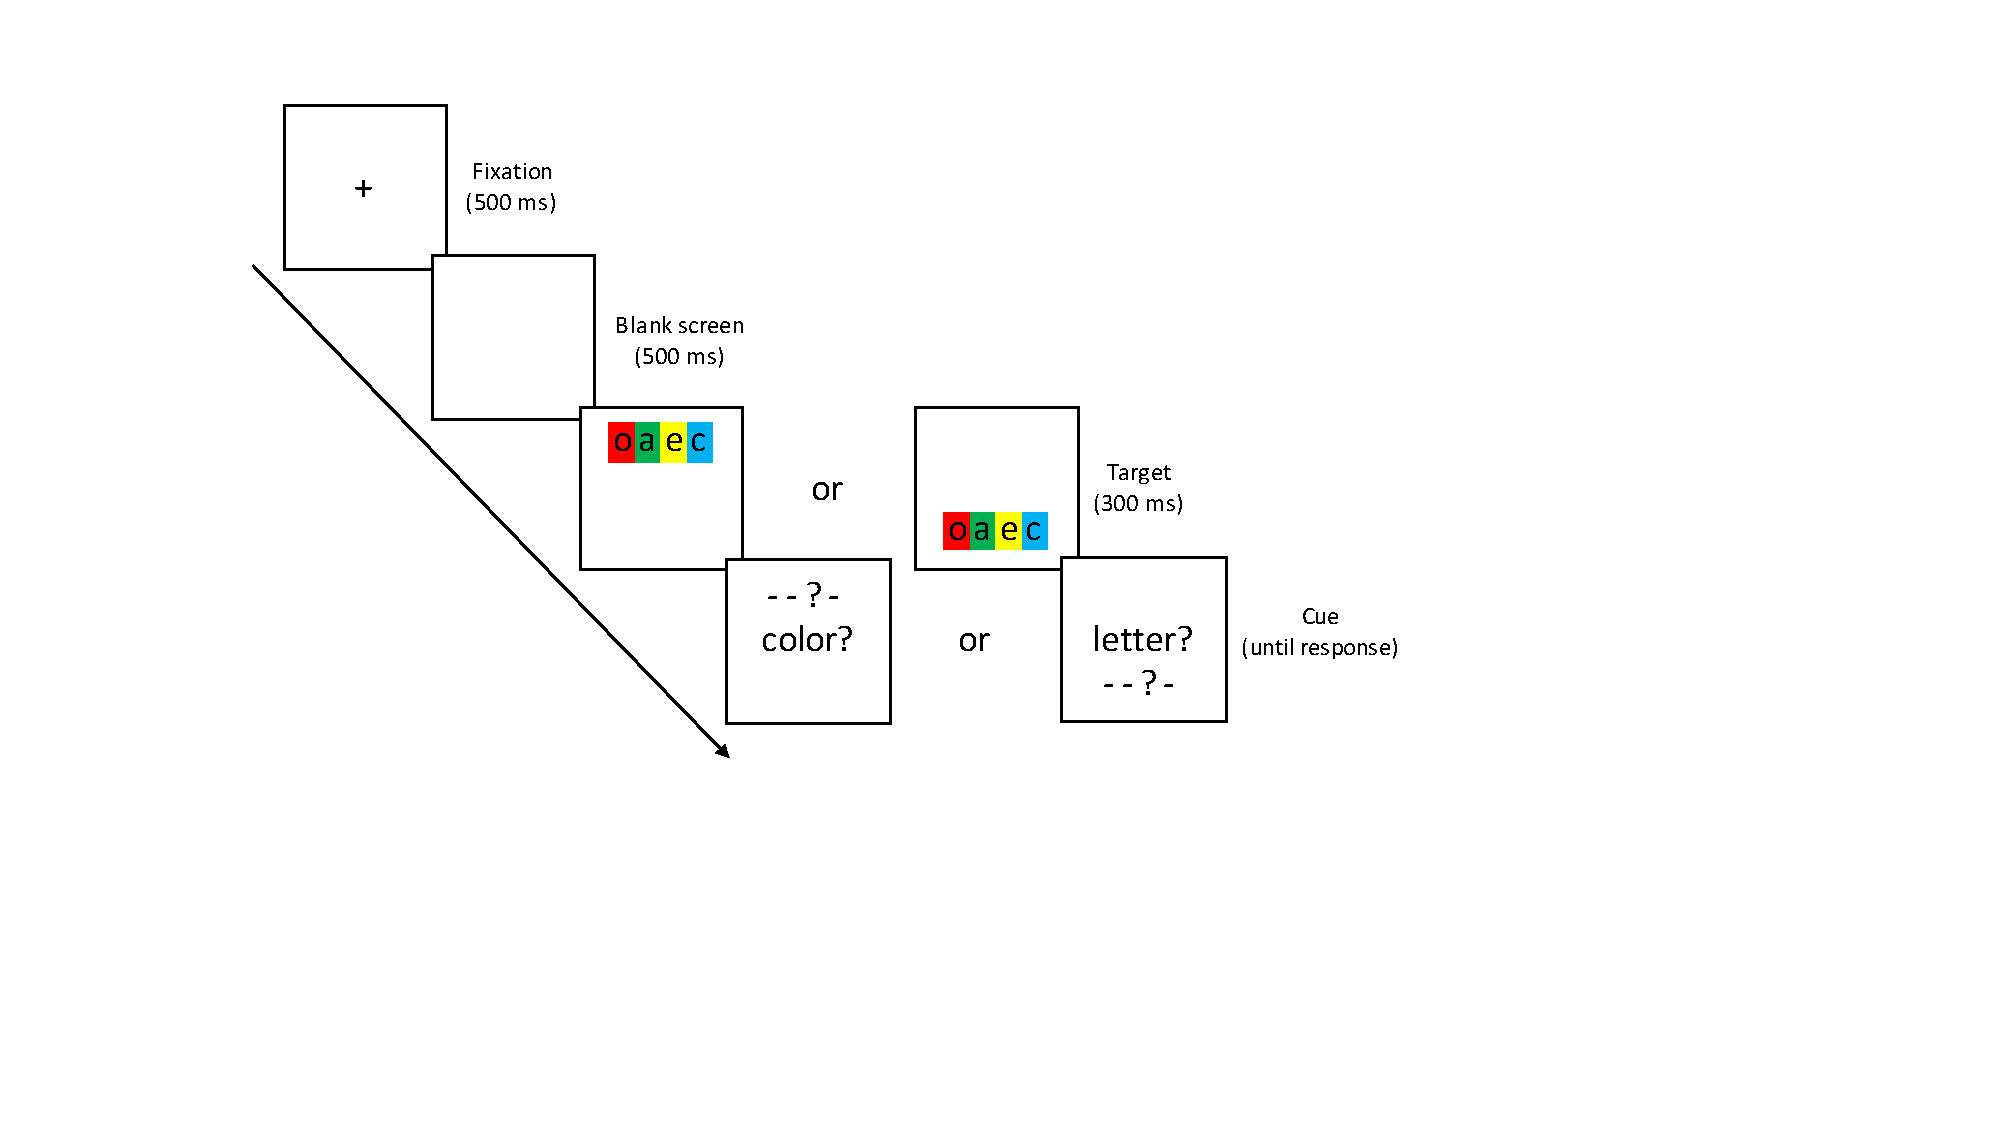
\includegraphics[width=5in]{figures/figure1.pdf}
  \caption{Illustration of the trial sequence for all experiments.}
  \caption*{Note that the target could appear above or below the fixation. The identity cue ("Color?" or "Letter?") always appeared in the center of the screen while the position cue ("- - ? -") always appeared in the same location as the target. Participants were instructed to report either the letter or color in the cued position.}

  \label{figure1}
\end{figure}

\hypertarget{section-2}{%
\section{Section 2}\label{section-2}}

Typically, a high proportion congruent experiment produces large
congruency effects, whereas a low proportion congruent experiment
produces small congruency effects (Logan and Zbrodoff, 1979; Lowe and
Mitterer, 1982; West and Baylis, 1998). This result is usually explained
as strategic control, where participants increase attentional control
under high-conflict demands and relax attentional control under
low-conflict demands (Logan, 1980; Logan and Zbrodoff, 1979; Logan,
Zbrodoff, and Williamson, 1984; Lowe and Mitterer, 1982).

\hypertarget{sub-section}{%
\subsection{Sub section}\label{sub-section}}

Recent work however, has demonstrated that attentional control is not
only adjusted by top-down regulation, but can also be triggered
automatically by environmental cues (Brosowsky and Crump, 2018; Bugg and
Crump, 2012; Egner, 2014; Fischer and Dreisbach, 2015; King, Korb, and
Egner, 2012; Mayr and Bryck, 2007).

\lipsum[1-9]

\FloatBarrier

\newpage
\fancyhead[L]{Chapter 2: running header}
\fancyhead[R]{\thepage}
\fancyfoot[C]{}

\chapter{Chapter 2: This chapter includes a latex table}

\lipsum[1-4]

\begin{table}[htbp]
  \centering
  \caption{Add caption}
  \resizebox{\textwidth}{!}{
    \begin{tabular}{rrcccccc}
    \toprule &  
    & \multicolumn{4}{c}{ Trial \textit{n}} 
    & \multicolumn{1}{c}{ Congruency Effect } 
    & \multicolumn{1}{c}{ $\textit{n}-1$ CSE} \\
    \cmidrule{3-6} &       
    & \multicolumn{2}{c}{ Con} 
    & \multicolumn{2}{c}{ Inc} 
    & \multicolumn{1}{c}{ $(I-C)$} 
    & \multicolumn{1}{c}{ ($C_{(I-C)} - I_{(I-C)})$} \\
    \cmidrule{3-8}
    & \multicolumn{1}{c}{ Trial $\textit{n}-1$} 
    & \multicolumn{1}{c}{ \textit{RT}} 
    & \multicolumn{1}{c}{ \textit{ER}} 
    & \multicolumn{1}{c}{ \textit{RT}} 
    & \multicolumn{1}{c}{ \textit{ER}} 
    & \multicolumn{1}{c}{ \textit{RT}} 
    & \multicolumn{1}{c}{ \textit{RT}} \\
    \midrule
    \multicolumn{2}{c}{\textbf{Exp. 1A}}  &   &    &     &     &    &  \\
    & \multicolumn{1}{c}{Con} 
    & \multicolumn{1}{c}{626 (22)} 
    & \multicolumn{1}{c}{2.97 (.55)} 
    & \multicolumn{1}{c}{658 (22)} 
    & \multicolumn{1}{c}{3.48 (.48)}
    & \multicolumn{1}{c}{32 (7)} 
    & \multicolumn{1}{c}{-3 (13)} \\
    & \multicolumn{1}{c}{Inc} 
    & \multicolumn{1}{c}{635 (21)} 
    & \multicolumn{1}{c}{3.55 (.46)} 
    & \multicolumn{1}{c}{671 (25)} 
    & \multicolumn{1}{c}{4.48 (.72)} 
    & \multicolumn{1}{c}{36 (9)} &  \\
    \multicolumn{2}{c}{\textbf{Exp. 1B}} &    &     &     &     &     &  \\
    & \multicolumn{1}{c}{Con} 
    & \multicolumn{1}{c}{753 (21)} 
    & \multicolumn{1}{c}{2.40 (.51)} 
    & \multicolumn{1}{c}{832 (25)} 
    & \multicolumn{1}{c}{3.48 (.53)} 
    & \multicolumn{1}{c}{78 (10)} 
    & \multicolumn{1}{c}{36 (12)} \\
    & \multicolumn{1}{c}{Inc}
    & \multicolumn{1}{c}{791 (24)} 
    & \multicolumn{1}{c}{3.58 (.54)} 
    & \multicolumn{1}{c}{671 (25)}
    & \multicolumn{1}{c}{3.23 (.71)} 
    & \multicolumn{1}{c}{42 (14)} &  \\
    \multicolumn{2}{c}{\textbf{Exp. 1C}} &       &       &       &       &       &  \\
    & \multicolumn{1}{c}{Con} 
    & \multicolumn{1}{c}{771 (27)} 
    & \multicolumn{1}{c}{2.46 (.37)} 
    & \multicolumn{1}{c}{834 (27)} 
    & \multicolumn{1}{c}{2.66 (.39)} 
    & \multicolumn{1}{c}{62 (6)} 
    & \multicolumn{1}{c}{27 (7)} \\
    & \multicolumn{1}{c}{Inc} 
    & \multicolumn{1}{c}{794 (25)} 
    & \multicolumn{1}{c}{2.91 (.40)} 
    & \multicolumn{1}{c}{829 (26)} 
    & \multicolumn{1}{c}{2.65 (.38)} 
    & \multicolumn{1}{c}{35 (7)} &  \\
    &       &       &       &       &       &       &  \\
    \midrule
    \multicolumn{2}{c}{\textbf{Exp. 2A}} &       &       &       &       &       &  \\
    & \multicolumn{1}{c}{Con} 
    & \multicolumn{1}{c}{557 (17)} 
    & \multicolumn{1}{c}{2.36 (.38)} 
    & \multicolumn{1}{c}{593 (16)} 
    & \multicolumn{1}{c}{4.36 (.57)} 
    & \multicolumn{1}{c}{36 (6)} 
    & \multicolumn{1}{c}{8 (8)} \\
    & \multicolumn{1}{c}{Inc} 
    & \multicolumn{1}{c}{576 (18)} 
    & \multicolumn{1}{c}{3.59 (.47)} 
    & \multicolumn{1}{c}{605 (19)} 
    & \multicolumn{1}{c}{3.80 (.60)} 
    & \multicolumn{1}{c}{28 (6)} &  \\
    \multicolumn{2}{c}{\textbf{Exp. 2B}} &       &       &       &       &       &  \\
    & \multicolumn{1}{c}{Con} 
    & \multicolumn{1}{c}{568 (20)} 
    & \multicolumn{1}{c}{1.91 (.37)} 
    & \multicolumn{1}{c}{638 (24)} 
    & \multicolumn{1}{c}{4.67 (.61)} 
    & \multicolumn{1}{c}{70 (5)} 
    & \multicolumn{1}{c}{33 (6)} \\
    & \multicolumn{1}{c}{Inc} 
    & \multicolumn{1}{c}{606 (24)} 
    & \multicolumn{1}{c}{2.83 (.41)} 
    & \multicolumn{1}{c}{643 (23)} 
    & \multicolumn{1}{c}{3.78 (.58)} 
    & \multicolumn{1}{c}{37 (7)} &  \\
    &       &       &       &       &       &       &  \\
    \midrule
    \multicolumn{2}{c}{\textbf{Exp. 3A}} &       &       &       &       &       &  \\
    & \multicolumn{1}{c}{Con} 
    & \multicolumn{1}{c}{837 (24)} 
    & \multicolumn{1}{c}{2.18 (.45)} 
    & \multicolumn{1}{c}{880 (20)} 
    & \multicolumn{1}{c}{2.65 (.41)} 
    & \multicolumn{1}{c}{43 (8)}
    & \multicolumn{1}{c}{22 (12)} \\
    & \multicolumn{1}{c}{Inc} 
    & \multicolumn{1}{c}{855 (21)} 
    & \multicolumn{1}{c}{2.83 (.40)} 
    & \multicolumn{1}{c}{876 (22)} 
    & \multicolumn{1}{c}{2.85 (.56)} 
    & \multicolumn{1}{c}{20 (8)} &  \\
    \multicolumn{2}{c}{\textbf{Exp. 3B}} &       &       &       &       &       &  \\
    & \multicolumn{1}{c}{Con} 
    & \multicolumn{1}{c}{860 (23)} 
    & \multicolumn{1}{c}{2.54 (.38)} 
    & \multicolumn{1}{c}{889 (24)} 
    & \multicolumn{1}{c}{2.38 (.42)} 
    & \multicolumn{1}{c}{30 (7)} 
    & \multicolumn{1}{c}{13 (10)} \\
    & \multicolumn{1}{c}{Inc} 
    & \multicolumn{1}{c}{873 (24)} 
    & \multicolumn{1}{c}{2.28 (.36)} 
    & \multicolumn{1}{c}{889 (23)} 
    & \multicolumn{1}{c}{2.43 (.35)} 
    & \multicolumn{1}{c}{16 (8)} &  \\
    &       &       &       &       &       &       &  \\
    \bottomrule
    \multicolumn{8}{l}{\textit{Note}: This is the note info} \\
    \end{tabular}}%
  \label{tab:addlabel}%
\end{table}

\FloatBarrier

\newpage
\fancyhead[L]{Chapter 3's Title}
\fancyhead[R]{\thepage}
\fancyfoot[C]{}

\chapter{Chapter 3's Title}

Don't stop now.

\FloatBarrier
\newpage
\fancyhead[L]{Chapter 4's Title}
\fancyhead[R]{\thepage}
\fancyfoot[C]{}

\chapter{Chapter 4's Title}

Keep it going.

\FloatBarrier
\newpage
\fancyhead[L]{Chapter 5's Title}
\fancyhead[R]{\thepage}
\fancyfoot[C]{}

\chapter{Chapter 5's Title}

Well done.

\FloatBarrier
\newpage

\fancyhead[L]{References}
\fancyhead[R]{\thepage}
\fancyfoot[C]{}

\chapter*{REFERENCES}

\setlength{\parindent}{-0.5in}
\setlength{\leftskip}{0.5in}
\setlength{\parskip}{6pt}

\noindent

\hypertarget{refs}{}
\leavevmode\hypertarget{ref-brosowsky_memory-guided_2018}{}%
Brosowsky, N. P., and Crump, M. J. C. (2018). Memory-guided selective
attention: Single experiences with conflict have long-lasting effects on
cognitive control. \emph{Journal of Experimental Psychology: General}.
\url{https://doi.org/10.1037/xge0000431}

\leavevmode\hypertarget{ref-bugg_support_2012}{}%
Bugg, J. M., and Crump, M. J. (2012). In support of a distinction
between voluntary and stimulus-driven control: A review of the
literature on proportion congruent effects. \emph{Frontiers in
Psychology}, \emph{3}, 367.
\url{https://doi.org/10.3389/fpsyg.2012.00367}

\leavevmode\hypertarget{ref-egner_creatures_2014}{}%
Egner, T. (2014). Creatures of habit (and control): A multi-level
learning perspective on the modulation of congruency effects.
\emph{Frontiers in Psychology}, \emph{5}, 1247.
\url{https://doi.org/10.3389/fpsyg.2014.01247}

\leavevmode\hypertarget{ref-eriksen_effects_1974}{}%
Eriksen, B. A., and Eriksen, C. W. (1974). Effects of noise letters upon
the identification of a target letter in a nonsearch task.
\emph{Perception \& Psychophysics}, \emph{16}, 143--149.
\url{https://doi.org/10.3758/BF03203267}

\leavevmode\hypertarget{ref-fischer_predicting_2015}{}%
Fischer, R., and Dreisbach, G. (2015). Predicting high levels of
multitasking reduces between-tasks interactions. Retrieved from
\url{http://psycnet.apa.org/psycinfo/2015-47211-001/}

\leavevmode\hypertarget{ref-king_priming_2012}{}%
King, J. A., Korb, F. M., and Egner, T. (2012). Priming of control:
Implicit contextual cuing of top-down attentional set. \emph{The Journal
of Neuroscience}, \emph{32}, 8192--8200.
\url{https://doi.org/10.1523/JNEUROSCI.0934-12.2012}

\leavevmode\hypertarget{ref-logan_attention_1980}{}%
Logan, G. D. (1980). Attention and automaticity in Stroop and priming
tasks: Theory and data. \emph{Cognitive Psychology}, \emph{12}(4),
523--553.

\leavevmode\hypertarget{ref-logan_when_1979}{}%
Logan, G. D., and Zbrodoff, N. J. (1979). When it helps to be misled:
Facilitative effects of increasing the frequency of conflicting stimuli
in a Stroop-like task. \emph{Memory \& Cognition}, \emph{7}, 166--174.
\url{https://doi.org/10.3758/BF03197535}

\leavevmode\hypertarget{ref-logan_strategies_1984}{}%
Logan, G. D., Zbrodoff, N. J., and Williamson, J. (1984). Strategies in
the color-word Stroop task. \emph{Bulletin of the Psychonomic Society},
\emph{22}(2), 135--138.

\leavevmode\hypertarget{ref-lowe_selective_1982}{}%
Lowe, D. G., and Mitterer, J. O. (1982). Selective and divided Attention
in a Stroop task. \emph{Canadian Journal of Psychology/Revue Canadienne
de Psychologie}, \emph{36}(4), 684.

\leavevmode\hypertarget{ref-mayr_outsourcing_2007}{}%
Mayr, U., and Bryck, R. L. (2007). Outsourcing control to the
environment: Effects of stimulus/response locations on task selection.
\emph{Psychological Research}, \emph{71}(1), 107--116.
\url{https://doi.org/10.1007/s00426-005-0039-x}

\leavevmode\hypertarget{ref-stroop_studies_1935}{}%
Stroop, J. R. (1935). Studies of interference in serial verbal
reactions. \emph{Journal of Experimental Psychology}, \emph{18}, 643.
\url{https://doi.org/10.1037/h0054651}

\leavevmode\hypertarget{ref-west_effects_1998}{}%
West, R., and Baylis, G. C. (1998). Effects of increased response
dominance and contextual disintegration on the Stroop interference
effect in older adults. \emph{Psychology and Aging}, \emph{13}(2), 206.

\clearpage

\fancyhead[L]{Appendices}
\fancyhead[R]{\thepage}
\fancyfoot[C]{}
\chapter*{APPENDICES}
\addcontentsline{toc}{chapter}{APPENDICES}

\doublespacing

\hypertarget{appendix-a-r-code-for-chapter-5}{%
\section*{Appendix A: R Code for Chapter
5}\label{appendix-a-r-code-for-chapter-5}}
\addcontentsline{toc}{section}{Appendix A: R Code for Chapter 5}

\singlespace

Required: R Packages from CRAN

\small

\begin{Shaded}
\begin{Highlighting}[]
\ControlFlowTok{if}\NormalTok{ (}\OperatorTok{!}\KeywordTok{require}\NormalTok{(tidyverse))\{}
  \KeywordTok{install.packages}\NormalTok{(}\StringTok{"tidyverse"}\NormalTok{)}
  \KeywordTok{library}\NormalTok{(tidyverse)}
\NormalTok{\}}
\ControlFlowTok{if}\NormalTok{ (}\OperatorTok{!}\KeywordTok{require}\NormalTok{(furniture))\{}
  \KeywordTok{install.packages}\NormalTok{(}\StringTok{"furniture"}\NormalTok{)}
  \KeywordTok{library}\NormalTok{(furniture)}
\NormalTok{\}}
\ControlFlowTok{if}\NormalTok{ (}\OperatorTok{!}\KeywordTok{require}\NormalTok{(here))\{}
  \KeywordTok{install.packages}\NormalTok{(}\StringTok{"here"}\NormalTok{)}
  \KeywordTok{library}\NormalTok{(here)}
\NormalTok{\}}
\ControlFlowTok{if}\NormalTok{ (}\OperatorTok{!}\KeywordTok{require}\NormalTok{(devtools))\{}
  \KeywordTok{install.packages}\NormalTok{(}\StringTok{"devtools"}\NormalTok{)}
  \KeywordTok{library}\NormalTok{(devtools)}
\NormalTok{\}}
\end{Highlighting}
\end{Shaded}

\normalsize

Required: R Packages from GitHub

\small

\begin{Shaded}
\begin{Highlighting}[]
\ControlFlowTok{if}\NormalTok{ (}\OperatorTok{!}\KeywordTok{require}\NormalTok{(MarginalMediation))\{}
\NormalTok{  devtools}\OperatorTok{::}\KeywordTok{install_github}\NormalTok{(}\StringTok{"tysonstanley/MarginalMediation"}\NormalTok{)}
  \KeywordTok{library}\NormalTok{(MarginalMediation)}
\NormalTok{\}}
\end{Highlighting}
\end{Shaded}

\normalsize

\clearpage

\hypertarget{examples-from-chapter-5}{%
\subsection*{Examples from Chapter 5}\label{examples-from-chapter-5}}
\addcontentsline{toc}{subsection}{Examples from Chapter 5}

Figure \ref{fig:interaction} on page \pageref{fig:interaction}

\small

\normalsize

\clearpage

\hypertarget{monte-carlo-simulation}{%
\subsection*{Monte Carlo Simulation}\label{monte-carlo-simulation}}
\addcontentsline{toc}{subsection}{Monte Carlo Simulation}

Notably, the code for both the binary mediator condition and the count
mediator condition we run via the Terminal as, once the directory was
where the R file was located:

\small

\begin{Shaded}
\begin{Highlighting}[]
\ExtensionTok{Rscript}\NormalTok{ Analyses_MMMC_scriptBinary.R }\StringTok{'c(1:45)'}
\end{Highlighting}
\end{Shaded}

\normalsize

\noindent and

\small

\begin{Shaded}
\begin{Highlighting}[]
\ExtensionTok{Rscript}\NormalTok{ Analyses_MMMC_scriptCount.R }\StringTok{'c(1:45)'}
\end{Highlighting}
\end{Shaded}

\normalsize

Binary Mediator

\small

\begin{Shaded}
\begin{Highlighting}[]
\CommentTok{## Marginal Mediation: Monte Carlo Simulation Study}
\CommentTok{##   BINARY Mediator}
\CommentTok{## Tyson S. Barrett}
\CommentTok{##}
\CommentTok{## devtools::install_github("tysonstanley/MarginalMediation")}

\NormalTok{args <-}\StringTok{ }\KeywordTok{commandArgs}\NormalTok{(}\OtherTok{TRUE}\NormalTok{)}
\NormalTok{args <-}\StringTok{ }\KeywordTok{eval}\NormalTok{(}\KeywordTok{parse}\NormalTok{(}\DataTypeTok{text =}\NormalTok{ args))}
\KeywordTok{library}\NormalTok{(MarginalMediation)}
\KeywordTok{library}\NormalTok{(tidyverse)}

\CommentTok{## Create all combinations of independent variables}
\NormalTok{cond_binary <-}\StringTok{ }\KeywordTok{expand.grid}\NormalTok{(}
  \DataTypeTok{samplesize =} \KeywordTok{c}\NormalTok{(}\DecValTok{50}\NormalTok{, }\DecValTok{100}\NormalTok{, }\DecValTok{200}\NormalTok{, }\DecValTok{500}\NormalTok{, }\DecValTok{1000}\NormalTok{),}
  \DataTypeTok{effecta =} \KeywordTok{c}\NormalTok{(.}\DecValTok{55}\NormalTok{, }\FloatTok{1.45}\NormalTok{, }\FloatTok{2.22}\NormalTok{),}
  \DataTypeTok{effectb =} \KeywordTok{c}\NormalTok{(.}\DecValTok{24}\NormalTok{, }\FloatTok{.62}\NormalTok{, }\FloatTok{1.068}\NormalTok{),}
  \DataTypeTok{effectc =} \KeywordTok{c}\NormalTok{(.}\DecValTok{3}\NormalTok{)}
\NormalTok{)}

\CommentTok{## Population Models}
\CommentTok{## Binary Mediator}
\NormalTok{data_genB <-}\StringTok{ }\ControlFlowTok{function}\NormalTok{(ps, reps, samplesize, effecta, effectb, effectc) \{}
  \KeywordTok{set.seed}\NormalTok{(}\DecValTok{84322}\NormalTok{)}
\NormalTok{  Xc <-}\StringTok{ }\KeywordTok{rnorm}\NormalTok{(ps)}
\NormalTok{  z <-}\StringTok{ }\NormalTok{effecta }\OperatorTok{*}\StringTok{ }\NormalTok{Xc }\OperatorTok{+}\StringTok{ }\KeywordTok{rnorm}\NormalTok{(ps, }\DecValTok{0}\NormalTok{, }\DecValTok{1}\NormalTok{)}
\NormalTok{  pr <-}\StringTok{ }\DecValTok{1} \OperatorTok{/}\StringTok{ }\NormalTok{(}\DecValTok{1} \OperatorTok{+}\StringTok{ }\KeywordTok{exp}\NormalTok{(}\OperatorTok{-}\NormalTok{z))}
\NormalTok{  M <-}\StringTok{ }\KeywordTok{rbinom}\NormalTok{(ps, }\DecValTok{1}\NormalTok{, pr)}
\NormalTok{  Y <-}\StringTok{ }\NormalTok{effectb }\OperatorTok{*}\StringTok{ }\NormalTok{M }\OperatorTok{+}\StringTok{ }\NormalTok{effectc }\OperatorTok{*}\StringTok{ }\NormalTok{Xc }\OperatorTok{+}\StringTok{ }\KeywordTok{rnorm}\NormalTok{(ps, }\DecValTok{0}\NormalTok{, }\DecValTok{1}\NormalTok{)}
\NormalTok{  M <-}\StringTok{ }\KeywordTok{factor}\NormalTok{(M)}
\NormalTok{  df <-}\StringTok{ }\KeywordTok{data.frame}\NormalTok{(Y, M, Xc)}
\NormalTok{  bin <-}\StringTok{ }\KeywordTok{vector}\NormalTok{(}\StringTok{"list"}\NormalTok{, reps)}

  \KeywordTok{print}\NormalTok{(}\KeywordTok{cbind}\NormalTok{(samplesize, effecta, effectb))}
  \KeywordTok{print}\NormalTok{(}\KeywordTok{lm}\NormalTok{(Y }\OperatorTok{~}\StringTok{ }\NormalTok{M }\OperatorTok{+}\StringTok{ }\NormalTok{Xc)}\OperatorTok{$}\NormalTok{coefficients)}
  \KeywordTok{print}\NormalTok{(}\KeywordTok{lm}\NormalTok{(}\KeywordTok{scale}\NormalTok{(Y) }\OperatorTok{~}\StringTok{ }\NormalTok{M }\OperatorTok{+}\StringTok{ }\NormalTok{Xc)}\OperatorTok{$}\NormalTok{coefficients)}
\NormalTok{  med <-}\StringTok{ }\KeywordTok{amed}\NormalTok{(}\KeywordTok{glm}\NormalTok{(M }\OperatorTok{~}\StringTok{ }\NormalTok{Xc, df, }\DataTypeTok{family =} \StringTok{"binomial"}\NormalTok{))}

  \ControlFlowTok{for}\NormalTok{ (i }\ControlFlowTok{in} \DecValTok{1}\OperatorTok{:}\NormalTok{reps) \{}
\NormalTok{    d <-}\StringTok{ }\NormalTok{df[}\KeywordTok{sample}\NormalTok{(ps, samplesize), ]}
\NormalTok{    pathbc <-}\StringTok{ }\KeywordTok{glm}\NormalTok{(Y }\OperatorTok{~}\StringTok{ }\NormalTok{M }\OperatorTok{+}\StringTok{ }\NormalTok{Xc, }\DataTypeTok{data =}\NormalTok{ d)}
\NormalTok{    patha <-}\StringTok{ }\KeywordTok{glm}\NormalTok{(M }\OperatorTok{~}\StringTok{ }\NormalTok{Xc, }\DataTypeTok{data =}\NormalTok{ d, }\DataTypeTok{family =} \StringTok{"binomial"}\NormalTok{)}
\NormalTok{    bin[[i]] <-}\StringTok{ }\KeywordTok{mma}\NormalTok{(pathbc, patha,}
      \DataTypeTok{ind_effects =} \KeywordTok{c}\NormalTok{(}\StringTok{"Xc-M"}\NormalTok{),}
      \DataTypeTok{boot =} \DecValTok{500}
\NormalTok{    )}
\NormalTok{    bin[[i]] <-}\StringTok{ }\KeywordTok{list}\NormalTok{(}
      \StringTok{"IndEffects"}\NormalTok{ =}\StringTok{ }\NormalTok{bin[[i]]}\OperatorTok{$}\NormalTok{ind_effects,}
      \StringTok{"DirEffects"}\NormalTok{ =}\StringTok{ }\NormalTok{bin[[i]]}\OperatorTok{$}\NormalTok{dir_effects,}
      \StringTok{"Boot"}\NormalTok{ =}\StringTok{ }\NormalTok{bin[[i]]}\OperatorTok{$}\NormalTok{boot,}
      \StringTok{"Total"}\NormalTok{ =}\StringTok{ }\KeywordTok{lm}\NormalTok{(Y }\OperatorTok{~}\StringTok{ }\NormalTok{Xc, d)}\OperatorTok{$}\NormalTok{coefficients,}
      \StringTok{"MedSize"}\NormalTok{ =}\StringTok{ }\NormalTok{med}
\NormalTok{    )}
    \KeywordTok{cat}\NormalTok{(}\StringTok{"}\CharTok{\textbackslash{}r}\StringTok{"}\NormalTok{, i)}
\NormalTok{  \}}
  \KeywordTok{print}\NormalTok{(}\KeywordTok{exp}\NormalTok{(}\KeywordTok{glm}\NormalTok{(M }\OperatorTok{~}\StringTok{ }\NormalTok{Xc, }\DataTypeTok{family =} \StringTok{"binomial"}\NormalTok{)}\OperatorTok{$}\NormalTok{coefficients))}
  \KeywordTok{return}\NormalTok{(bin)}
\NormalTok{\}}

\NormalTok{i =}\StringTok{ }\DecValTok{0}
\ControlFlowTok{for}\NormalTok{ (j }\ControlFlowTok{in}\NormalTok{ args)\{}
  \KeywordTok{set.seed}\NormalTok{(}\DecValTok{84322}\NormalTok{)}
\NormalTok{  i =}\StringTok{ }\NormalTok{i }\OperatorTok{+}\StringTok{ }\DecValTok{1}
  \KeywordTok{cat}\NormalTok{(}\StringTok{"}\CharTok{\textbackslash{}n}\StringTok{Number:"}\NormalTok{, j, }\StringTok{"}\CharTok{\textbackslash{}n\textbackslash{}n}\StringTok{"}\NormalTok{)}
  
\NormalTok{  out =}\StringTok{ }\KeywordTok{data_genB}\NormalTok{(}\FloatTok{1e6}\NormalTok{, }\DecValTok{500}\NormalTok{, }
\NormalTok{                  cond_binary[args[[i]],}\DecValTok{1}\NormalTok{], }
\NormalTok{                  cond_binary[args[[i]],}\DecValTok{2}\NormalTok{], }
\NormalTok{                  cond_binary[args[[i]],}\DecValTok{3}\NormalTok{], }
\NormalTok{                  cond_binary[args[[i]],}\DecValTok{4}\NormalTok{])}
  
  \KeywordTok{save}\NormalTok{(out, }\DataTypeTok{file =} \KeywordTok{paste0}\NormalTok{(}\StringTok{"Sims_Data/Binary2_"}\NormalTok{, }
\NormalTok{                          cond_binary[args[[i]],}\DecValTok{1}\NormalTok{], }\StringTok{"_"}\NormalTok{,}
\NormalTok{                          cond_binary[args[[i]],}\DecValTok{2}\NormalTok{], }\StringTok{"_"}\NormalTok{,}
\NormalTok{                          cond_binary[args[[i]],}\DecValTok{3}\NormalTok{], }\StringTok{"_"}\NormalTok{,}
\NormalTok{                          cond_binary[args[[i]],}\DecValTok{4}\NormalTok{], }\StringTok{".rda"}\NormalTok{))}
  
  \KeywordTok{cat}\NormalTok{(}\StringTok{"}\CharTok{\textbackslash{}n}\StringTok{Number:"}\NormalTok{, j, }\StringTok{"}\CharTok{\textbackslash{}n\textbackslash{}n}\StringTok{"}\NormalTok{)}
  \KeywordTok{cat}\NormalTok{(}\StringTok{"}\CharTok{\textbackslash{}n}\StringTok{Conditions Complete:}\CharTok{\textbackslash{}n}\StringTok{"}\NormalTok{,}
      \StringTok{" Sample size ="}\NormalTok{, cond_binary[args[[i]],}\DecValTok{1}\NormalTok{], }
      \StringTok{"}\CharTok{\textbackslash{}n}\StringTok{  A path      ="}\NormalTok{, cond_binary[args[[i]],}\DecValTok{2}\NormalTok{], }
      \StringTok{"}\CharTok{\textbackslash{}n}\StringTok{  B path      ="}\NormalTok{, cond_binary[args[[i]],}\DecValTok{3}\NormalTok{], }
      \StringTok{"}\CharTok{\textbackslash{}n}\StringTok{  C path      ="}\NormalTok{, cond_binary[args[[i]],}\DecValTok{4}\NormalTok{], }\StringTok{"}\CharTok{\textbackslash{}n}\StringTok{"}\NormalTok{)}
\NormalTok{\}}
\end{Highlighting}
\end{Shaded}

\normalsize

Count Mediator

\small

\begin{Shaded}
\begin{Highlighting}[]
\CommentTok{## Marginal Mediation: Monte Carlo Simulation Study}
\CommentTok{##   COUNT Mediator}
\CommentTok{## Tyson S. Barrett}
\CommentTok{##}
\CommentTok{## devtools::install_github("tysonstanley/MarginalMediation")}

\NormalTok{args <-}\StringTok{ }\KeywordTok{commandArgs}\NormalTok{(}\OtherTok{TRUE}\NormalTok{)}
\NormalTok{args <-}\StringTok{ }\KeywordTok{eval}\NormalTok{(}\KeywordTok{parse}\NormalTok{(}\DataTypeTok{text =}\NormalTok{ args))}
\KeywordTok{library}\NormalTok{(MarginalMediation)}
\KeywordTok{library}\NormalTok{(tidyverse)}

\CommentTok{## Create all combinations of independent variables}
\NormalTok{cond_count =}\StringTok{ }\KeywordTok{expand.grid}\NormalTok{(}
  \DataTypeTok{samplesize =} \KeywordTok{c}\NormalTok{(}\DecValTok{50}\NormalTok{, }\DecValTok{100}\NormalTok{, }\DecValTok{200}\NormalTok{, }\DecValTok{500}\NormalTok{, }\DecValTok{1000}\NormalTok{),}
  \DataTypeTok{effecta    =} \KeywordTok{c}\NormalTok{(.}\DecValTok{3}\NormalTok{, }\FloatTok{.6}\NormalTok{, }\FloatTok{1.1}\NormalTok{),}
  \DataTypeTok{effectb    =} \KeywordTok{c}\NormalTok{(.}\DecValTok{084}\NormalTok{, }\FloatTok{.265}\NormalTok{, }\FloatTok{.49}\NormalTok{),}
  \DataTypeTok{effectc    =} \KeywordTok{c}\NormalTok{(}\DecValTok{0}\NormalTok{, }\FloatTok{.3}\NormalTok{)}
\NormalTok{)}

\CommentTok{## Population Models}
\CommentTok{## Count Mediator}
\NormalTok{data_genC =}\StringTok{ }\ControlFlowTok{function}\NormalTok{(ps, reps, samplesize, effecta, effectb, effectc)\{}
  \KeywordTok{set.seed}\NormalTok{(}\DecValTok{84322}\NormalTok{)}
\NormalTok{  Xc =}\StringTok{ }\KeywordTok{rnorm}\NormalTok{(ps)}
\NormalTok{  m1 =}\StringTok{ }\KeywordTok{exp}\NormalTok{(effecta }\OperatorTok{*}\StringTok{ }\NormalTok{Xc)}
\NormalTok{  M  =}\StringTok{ }\KeywordTok{rpois}\NormalTok{(ps, }\DataTypeTok{lambda=}\NormalTok{m1)}
\NormalTok{  Y  =}\StringTok{ }\NormalTok{effectb}\OperatorTok{*}\NormalTok{M }\OperatorTok{+}\StringTok{ }\NormalTok{effectc}\OperatorTok{*}\NormalTok{Xc }\OperatorTok{+}\StringTok{ }\KeywordTok{rnorm}\NormalTok{(ps, }\DecValTok{0}\NormalTok{, }\DecValTok{1}\NormalTok{)}
\NormalTok{  df =}\StringTok{ }\KeywordTok{data.frame}\NormalTok{(Y, M, Xc)}
\NormalTok{  poi  =}\StringTok{ }\KeywordTok{vector}\NormalTok{(}\StringTok{"list"}\NormalTok{, reps)}
  
  \KeywordTok{print}\NormalTok{(}\KeywordTok{cbind}\NormalTok{(samplesize, effecta, effectb))}
  \KeywordTok{print}\NormalTok{(}\KeywordTok{lm}\NormalTok{(Y }\OperatorTok{~}\StringTok{ }\NormalTok{M }\OperatorTok{+}\StringTok{ }\NormalTok{Xc)}\OperatorTok{$}\NormalTok{coefficients)}
  \KeywordTok{print}\NormalTok{(}\KeywordTok{lm}\NormalTok{(}\KeywordTok{scale}\NormalTok{(Y) }\OperatorTok{~}\StringTok{ }\NormalTok{M }\OperatorTok{+}\StringTok{ }\NormalTok{Xc)}\OperatorTok{$}\NormalTok{coefficients)}
\NormalTok{  med =}\StringTok{ }\KeywordTok{amed}\NormalTok{(}\KeywordTok{glm}\NormalTok{(M }\OperatorTok{~}\StringTok{ }\NormalTok{Xc, df, }\DataTypeTok{family =} \StringTok{"poisson"}\NormalTok{))}
  
  \ControlFlowTok{for}\NormalTok{ (i }\ControlFlowTok{in} \DecValTok{1}\OperatorTok{:}\NormalTok{reps)\{}
\NormalTok{    d =}\StringTok{ }\NormalTok{df[}\KeywordTok{sample}\NormalTok{(ps, samplesize), ]}
\NormalTok{    pathbc =}\StringTok{ }\KeywordTok{glm}\NormalTok{(Y }\OperatorTok{~}\StringTok{ }\NormalTok{M }\OperatorTok{+}\StringTok{ }\NormalTok{Xc, }\DataTypeTok{data =}\NormalTok{ d)}
\NormalTok{    patha  =}\StringTok{ }\KeywordTok{glm}\NormalTok{(M }\OperatorTok{~}\StringTok{ }\NormalTok{Xc, }\DataTypeTok{data =}\NormalTok{ d, }\DataTypeTok{family =} \StringTok{"poisson"}\NormalTok{)}
\NormalTok{    poi[[i]] =}\StringTok{ }\KeywordTok{mma}\NormalTok{(pathbc, patha,}
                   \DataTypeTok{ind_effects =} \KeywordTok{c}\NormalTok{(}\StringTok{"Xc-M"}\NormalTok{),}
                   \DataTypeTok{boot =} \DecValTok{500}\NormalTok{)}
\NormalTok{    poi[[i]] =}\StringTok{ }\KeywordTok{list}\NormalTok{(}\StringTok{"IndEffects"}\NormalTok{ =}\StringTok{ }\NormalTok{poi[[i]]}\OperatorTok{$}\NormalTok{ind_effects, }
                    \StringTok{"DirEffects"}\NormalTok{ =}\StringTok{ }\NormalTok{poi[[i]]}\OperatorTok{$}\NormalTok{dir_effects, }
                    \StringTok{"Boot"}\NormalTok{       =}\StringTok{ }\NormalTok{poi[[i]]}\OperatorTok{$}\NormalTok{boot, }
                    \StringTok{"Total"}\NormalTok{      =}\StringTok{ }\KeywordTok{lm}\NormalTok{(Y }\OperatorTok{~}\StringTok{ }\NormalTok{Xc, d)}\OperatorTok{$}\NormalTok{coefficients,}
                    \StringTok{"MedSize"}\NormalTok{    =}\StringTok{ }\NormalTok{med)}
    \KeywordTok{cat}\NormalTok{(}\StringTok{"}\CharTok{\textbackslash{}r}\StringTok{"}\NormalTok{, i)}
\NormalTok{  \}}
  \KeywordTok{print}\NormalTok{(}\KeywordTok{exp}\NormalTok{(}\KeywordTok{glm}\NormalTok{(M }\OperatorTok{~}\StringTok{ }\NormalTok{Xc, }\DataTypeTok{family =} \StringTok{"poisson"}\NormalTok{)}\OperatorTok{$}\NormalTok{coefficients))}
  \KeywordTok{return}\NormalTok{(poi)}
\NormalTok{\}}

\NormalTok{i =}\StringTok{ }\DecValTok{0}
\ControlFlowTok{for}\NormalTok{ (j }\ControlFlowTok{in}\NormalTok{ args)\{}
  \KeywordTok{set.seed}\NormalTok{(}\DecValTok{84322}\NormalTok{)}
\NormalTok{  i =}\StringTok{ }\NormalTok{i }\OperatorTok{+}\StringTok{ }\DecValTok{1}
  \KeywordTok{cat}\NormalTok{(}\StringTok{"}\CharTok{\textbackslash{}n}\StringTok{Number:"}\NormalTok{, j, }\StringTok{"}\CharTok{\textbackslash{}n\textbackslash{}n}\StringTok{"}\NormalTok{)}
  
\NormalTok{  out =}\StringTok{ }\KeywordTok{data_genC}\NormalTok{(}\FloatTok{1e6}\NormalTok{, }\DecValTok{500}\NormalTok{, }
\NormalTok{                  cond_count[args[[i]],}\DecValTok{1}\NormalTok{], }
\NormalTok{                  cond_count[args[[i]],}\DecValTok{2}\NormalTok{], }
\NormalTok{                  cond_count[args[[i]],}\DecValTok{3}\NormalTok{], }
\NormalTok{                  cond_count[args[[i]],}\DecValTok{4}\NormalTok{])}
  
  \KeywordTok{save}\NormalTok{(out, }\DataTypeTok{file =} \KeywordTok{paste0}\NormalTok{(}\StringTok{"Sims_Data/Count2_"}\NormalTok{, }
\NormalTok{                          cond_count[args[[i]],}\DecValTok{1}\NormalTok{], }\StringTok{"_"}\NormalTok{,}
\NormalTok{                          cond_count[args[[i]],}\DecValTok{2}\NormalTok{], }\StringTok{"_"}\NormalTok{,}
\NormalTok{                          cond_count[args[[i]],}\DecValTok{3}\NormalTok{], }\StringTok{"_"}\NormalTok{,}
\NormalTok{                          cond_count[args[[i]],}\DecValTok{4}\NormalTok{], }\StringTok{".rda"}\NormalTok{))}
  
  \KeywordTok{cat}\NormalTok{(}\StringTok{"}\CharTok{\textbackslash{}n}\StringTok{Number:"}\NormalTok{, j, }\StringTok{"}\CharTok{\textbackslash{}n\textbackslash{}n}\StringTok{"}\NormalTok{)}
  \KeywordTok{cat}\NormalTok{(}\StringTok{"}\CharTok{\textbackslash{}n}\StringTok{Conditions Complete:}\CharTok{\textbackslash{}n}\StringTok{"}\NormalTok{,}
      \StringTok{" Sample size ="}\NormalTok{, cond_count[args[[i]],}\DecValTok{1}\NormalTok{], }
      \StringTok{"}\CharTok{\textbackslash{}n}\StringTok{  A path      ="}\NormalTok{, cond_count[args[[i]],}\DecValTok{2}\NormalTok{], }
      \StringTok{"}\CharTok{\textbackslash{}n}\StringTok{  B path      ="}\NormalTok{, cond_count[args[[i]],}\DecValTok{3}\NormalTok{], }
      \StringTok{"}\CharTok{\textbackslash{}n}\StringTok{  C path      ="}\NormalTok{, cond_count[args[[i]],}\DecValTok{4}\NormalTok{], }\StringTok{"}\CharTok{\textbackslash{}n}\StringTok{"}\NormalTok{)}
\NormalTok{\}}
\end{Highlighting}
\end{Shaded}

\normalsize

\clearpage

\hypertarget{monte-carlo-simulation-data-analyses}{%
\subsection*{Monte Carlo Simulation Data
Analyses}\label{monte-carlo-simulation-data-analyses}}
\addcontentsline{toc}{subsection}{Monte Carlo Simulation Data Analyses}

Data Preparations for tables and figures around page
\pageref{tab_discrep}

\small

\normalsize

Table \ref{tab_discrep} on page \pageref{tab_discrep}

\small

\normalsize

Figure \ref{fig:totaltotal} on page \pageref{fig:totaltotal}

\small

\normalsize

Figures \ref{fig_power}, \ref{fig_acc}, and \ref{fig_ci} on pages
\pageref{fig_power}, \pageref{fig_acc}, and \pageref{fig_ci},
respectively.

\small

\normalsize


\end{document}
